% Compile with XeLaTeX or LuaLaTeX, repeat until the "Rerun" warning disappears (3 times the first time):
%   xelatex Slide_HPCA.tex   (or: latexmk -xelatex Slide_HPCA.tex)
\documentclass[aspectratio=169,t,10pt]{beamer} % với tỉ lệ 4:3 thì thay 169 bằng 43
\usepackage[vietnamese]{babel}   % nếu gõ tiếng anh xóa dòng này hoặc thay bằng english
\usepackage[european, siunitx]{circuitikz}

\usetheme{HPCA}

\title{Nghiên cứu ứng dụng bộ biến đổi đa mức MMC trong hệ thống năng lượng tái tạo}
\hpcadoctype{LUẬN VĂN THẠC SĨ KHOA HỌC}
\hpcainfo{Học viên:}{Phạm Chí Hiếu}
\hpcainfo{Cán bộ hướng dẫn:}{TS. Phạm Việt Phương}

\begin{document}

\hpcatitlepage

\hpcatoc{Contents}

\section{Giới thiệu chung}
\begin{frame}{Motor drive systems}
  \begin{itemize}
    \item Motor drive systems (BLDC, PMSM, SCIM, etc.) for industrial applications.
    \begin{itemize}
      \item HVLS applications
    \end{itemize}
  \end{itemize}
   \begin{figure}
      \centering
      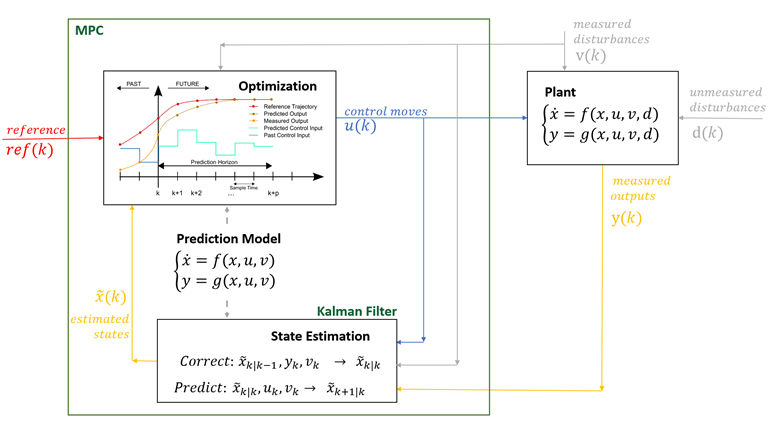
\includegraphics[width=0.6\linewidth]{images/image.png}
      \caption{Mô hình bộ MPC}
      \label{fig1}
  \end{figure}
\end{frame}

\section{Bộ biến đổi đa mức cấu trúc module - MMC}
\begin{frame}{Power electronics converters}
  \begin{itemize}
    \item Power electronics converters for renewable energy conversion systems.
    \begin{itemize}
      \item T-type converter
    \end{itemize}
     \begin{figure}
      \flushleft
      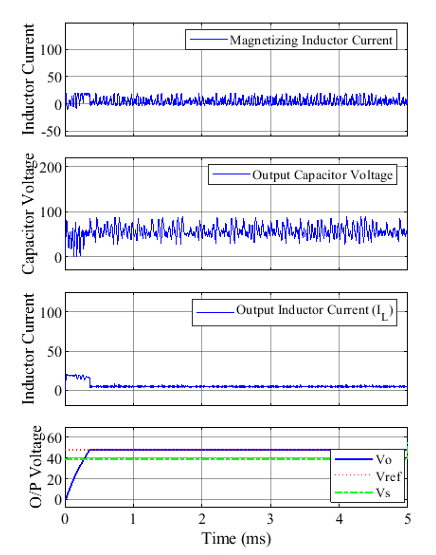
\includegraphics[width=0.3\linewidth]{images/image2.PNG}
      \caption{caption hình 2}
      \label{fig2}
  \end{figure}
  \end{itemize}

 từ \cite{vaswani2017attention} ta có
\end{frame}

\begin{frame}{Block và công thức}
  \begin{block}{Điện áp nhánh MMC}
    Điện áp mỗi nhánh là tổng điện áp các submodule đang được đưa vào mạch:
    \[ v_{arm} = \sum_{k=1}^{N} S_k\, v_{C,k} \]
  \end{block}

    \begin{figure}[scale=0.7]
        \centering
      \begin{circuitikz}
          \draw (0,0) to[R, l = $R_1$](4,0);
          \draw (0,-2) to[american inductor, l=$L_1$] (4,-2);
          \draw (0,0) to[sinusoidal voltage source, l=$AC$](0,-2);
          \draw (4,0) to[C, l=$C_1$](4,-2);
      \end{circuitikz}
        \caption{Hình vẽ mạch điện bằng circuitikz}
        \label{fig3}
    \end{figure}
\end{frame}

\section{Điều chế và cân bằng điện áp tụ điện Submodule}
\section{Điều khiển MMC nối lưới}
\section{Hệ thống truyền tải cao thế một chiều HVDC-MMC}
\section{Kết luận}

  % slide chia phần (chỉ có khối navy)

\begin{hpcaappendixframe}{Appendix}{Tài liệu tham khảo}   % slide phụ lục có nội dung

 \bibliographystyle{plain}
 \bibliography{ref}


\end{hpcaappendixframe}

\end{document}
